As discussed in Section \ref{sec:research} one of the possible paths for pivoting from pure publications or data repositories to research repositories consists of migrating records to a different system. Such a venture needs to be properly planned and executed in order to ensure, on one hand, that no records are lost or corrupted and, on the other hand, that minimal or no downtime is generated. Ideally, migrations would also be an opportunity to curate and enrich the existing corpus by consolidating and correcting bibliographic records. What differentiates such transfers from other data migrations is the required domain knowledge, the particularities of the target and source repositories in the context of the scholarly communications ecosystem, and the structure of the migration package, which includes, among others, bibliographic metadata, record files and usage data.

In this chapter a workflow and technical framework for performing repository migrations is discussed, based on the experience of six such transfers performed between 2018 and 2019. These considered records stored on various repository solutions (DSpace, Bepress Digital Commons), custom in-house built systems) that had to be moved to the Figshare \gls{saas} repository platform. For this purpose, SLAM (Stateful  Library  Analysis  and  Migration), an \gls{etl} system was developed and successfully employed in order to migrate over $80.000$ records. 

\newpage

\section{Background}
\label{sec:migbackground}

In early 2018 Figshare has started considering the suitability of its repository platform for storing, along with non-traditional research outputs (datasets or scientific software), content which is usually specific to \emph{institutional} repositories (journal articles, theses, monographs)\cite{fir}. While feature-wise this was validated by its hosted preprint servers\cite{chem}, a new challenge was posed, as clients choosing to use Figshare as an institutional repository also had to transfer all content from their existing systems.

Thus, in the first half of 2018, a first migration was performed, transferring records from a Bepress Digital Commons repository. From a technical point of view, a simple Python\footnote{\url{https://www.python.org/}} script was developed for this migration; this script parsed a \gls{csv} report produced by Digital Commons\cite{bepressdash} which contained all metadata and links to the record files\footnote{For records under embargo the files were transferred using a backchannel.}. Using this information, records were created on the Figshare repository using its \gls{api}\footnote{\url{https://api.figshare.com}}. While this migration succeeded, the \emph{naive} technical solution presented a number of issues:
\begin{itemize}
    \item Difficulties with the metadata crosswalk: while a crosswalk was initially set up, mostly based on the definition of the fields in the source and target repositories' schema\footnote{Both DC and Figshare use in-house custom metadata schemas which better fit their business and data model.}, issues were discovered while migrating the records, mainly due to inconsistencies in the values of the fields across the corpus. These issues were fixed on a case-by-case basis, in order to ensure a lossless migration, but it would have been preferred to surface them in the early phases, in order to have the migration script able to mitigate any issues in the final run.
    \item Difficulties in running the migration procedure multiple times: the migration script followed mostly an \emph{all or nothing} approach, where, at each run, it fully migrated all records between repositories. This was discovered to not be desirable, as there was a need to run the script only for those records that failed to migrate (due, for example, to metadata crosswalk issues). After the full migration was completed, there was also a need to apply only some minor corrections to records, without following the full procedure; this was not possible, due to the fact that the script would recreate all records to migrate from scratch on the target repository, as it did not have any \emph{memory} of previous runs\footnote{This issue was amplified by the fact that in the source repository records did not have any type of persistent identifier attached.}. Thus, additional scripts, which only performed the corrections, had to be developed.
    \item The migrations procedure required constant operator supervision: like most migrations, this instance considered a large number of records (over $10.000$) and, ideally, the migration procedure would run with minimal supervision required from operators. While the initial script partially accomplished this, needs for better fault-tolerance and enhanced logging were identified.
\end{itemize}

Given that a number of five other migrations were to be completed between October 2018 and December 2019, and the lessons learned from the initial attempt, it was required to develop a more robust alternative to the naive migration script; this alternative had to adhere to three main design principles:
\begin{enumerate}
    \item Reusability: the system should be usable for multiple migrations without extensive additions or modifications. Thus, it should be able to adapt to the workflows of multiple repositories, metadata schemas, and other concerns specific to each migration.
    \item Statefulness/ idempotence: the system should be able to perform the same migration multiple times, without creating duplicate records on the target repository, and allowing for incremental record improvements with each run. Apart from allowing for corrections to be applied post-migration, this would also support the prototyping phase, where multiple test migrations are performed in order to validate the metadata crosswalks, to verify that no information is lost, and other general workflow aspects.
    \item Fault tolerance: the system should implement fault tolerance mechanisms at all levels, allowing to run migrations of large corpora with minimal supervision, and, at the same time, implement sufficient logging and exception handling to allow operators to identify and correct potential issues.
\end{enumerate}

A number of repository migrations are present in the literature. In \cite{tragedy} the authors describe the process of moving from a DSpace to a Samvera\footnote{\url{https://samvera.org/}} system, while in \cite{challenges} the records were migrated from a solution developed in-house to DSpace. Both instances offer valuable insight into the challenges posed by digital library migrations, especially at the level of bibliographic metadata; on the other hand, both works are focused mostly on a specific use-case and do not propose general technical solutions for other migrations. It is interesting to note that the migration presented by \cite{tragedy} required $2.5$ years of work, while SLAM was employed to carry 5 migrations in 14 months.

The Bridge2Hyku toolkit\cite{bridge} is a collection of tools, including a module for the Hyku repository solution\footnote{\url{https://hyku.samvera.org/}}, aimed at facilitating the import of records into digital libraries based on this software. Similar to SLAM, it includes an analysis component, useful for surfacing and correcting potential metadata issues during the migration. SLAM provides two major improvements over this solution, namely it defines a generic architecture that can be used for migrating records between any two repositories, while also defining a procedural migration workflow in order to create a robust, fault-tolerant and extensible solution.

\subsection{Extract, transform, load}
\label{sec:etl}

\glsfirst{etl} is the process of transferring data between two systems which represent it in different formats or function in different contexts (e.g., on-premise versus cloud computing systems). An \gls{etl} system is able to extract data from one or multiple homogeneous or heterogeneous sources, to apply various operations in order to enforce quality and consistency standards and to deliver a presentation-ready format to the destination system(s).

Rising to popularity in the 1970s, \gls{etl} remains an integral part of \emph{data warehousing} pipelines, where data coming from multiple databases is aggregated in order to allow for analysis and reporting activities. With the advent of \emph{big data}, this workflow found new applicability, as it is advantageously positioned for implementing workloads that process large volumes of information that, most often, comes from disparate sources. One particularly notable result of this is the development of \emph{MapReduce}, a programming model that allows processing large data sets using a parallel, distributed algorithm on a cluster. In this model, the \emph{map} operation produces an intermediary value for each input, while \emph{reduce} aggregates all these values in order to produce the final results. The most popular implementation of this model is Hadoop\footnote{\url{https://hadoop.apache.org/}}, which allows running MapReduce workloads on commodity hardware.


\gls{etl} facilities have been also implemented by all major cloud computing providers, to name a few examples:
\begin{itemize}
    \item \gls{aws}: Glue\footnote{\url{https://aws.amazon.com/glue/}} is a fully managed \gls{etl} service, which can connect to various data sources (relational databases, file or objects storages) and allow users to define transformations using a high-level language such as Python. Other features include the the possibility to define recurring jobs, dependencies, automatic scaling or exception handling. 
    
    \item \gls{gcp}: in \cite{gcp} the authors outline an \gls{etl} framework built using a number of Google services; Cloud Dataflow\footnote{\url{https://cloud.google.com/dataflow}} is employed in order to aggregate data from different sources and BigQuery\footnote{\url{https://cloud.google.com/bigquery}} provides the transform, analysis and reporting operations, including visualisations for the data.
    
    \item Microsoft Azure: the Data Factory\footnote{\url{https://azure.microsoft.com/en-us/services/data-factory/}} service provides the building blocks for defining \gls{etl} workloads, including the ability to define operations both visually and by programming them in a language such as Python. Two points differentiate this service from the two options above: the use of open source technologies, such as Apache Spark, and the possibility to connect to external services, such as \gls{aws} file storages or \gls{gcp} BigQuery. This can facilitate the setup of workloads for engineers accustomed with other services and tools.
\end{itemize}

\gls{etl} finds applicability in scientific research, especially in areas such as life sciences or machine learning, where large volumes of data need to be processed in order to extract valuable information. For example, in \cite{denney} and \cite{godihno} the authors apply \gls{etl} workloads in order to analyse clinical records, while in \cite{ferreira} such a system in devised in order to discover and aggregate citations in an \gls{ir}.

\section{SLAM: the Stateful  Library  Analysis  and  Migration framework}
\label{sec:slam}

Following the design principles mentioned previously, SLAM's architecture was devised as presented in Fig. \ref{fig:workflow}; as it is an \gls{etl} system, the easiest way of understanding its operation is by examining the data flow.

\begin{sidewaysfigure}[ht!]
  \centering
  \fbox{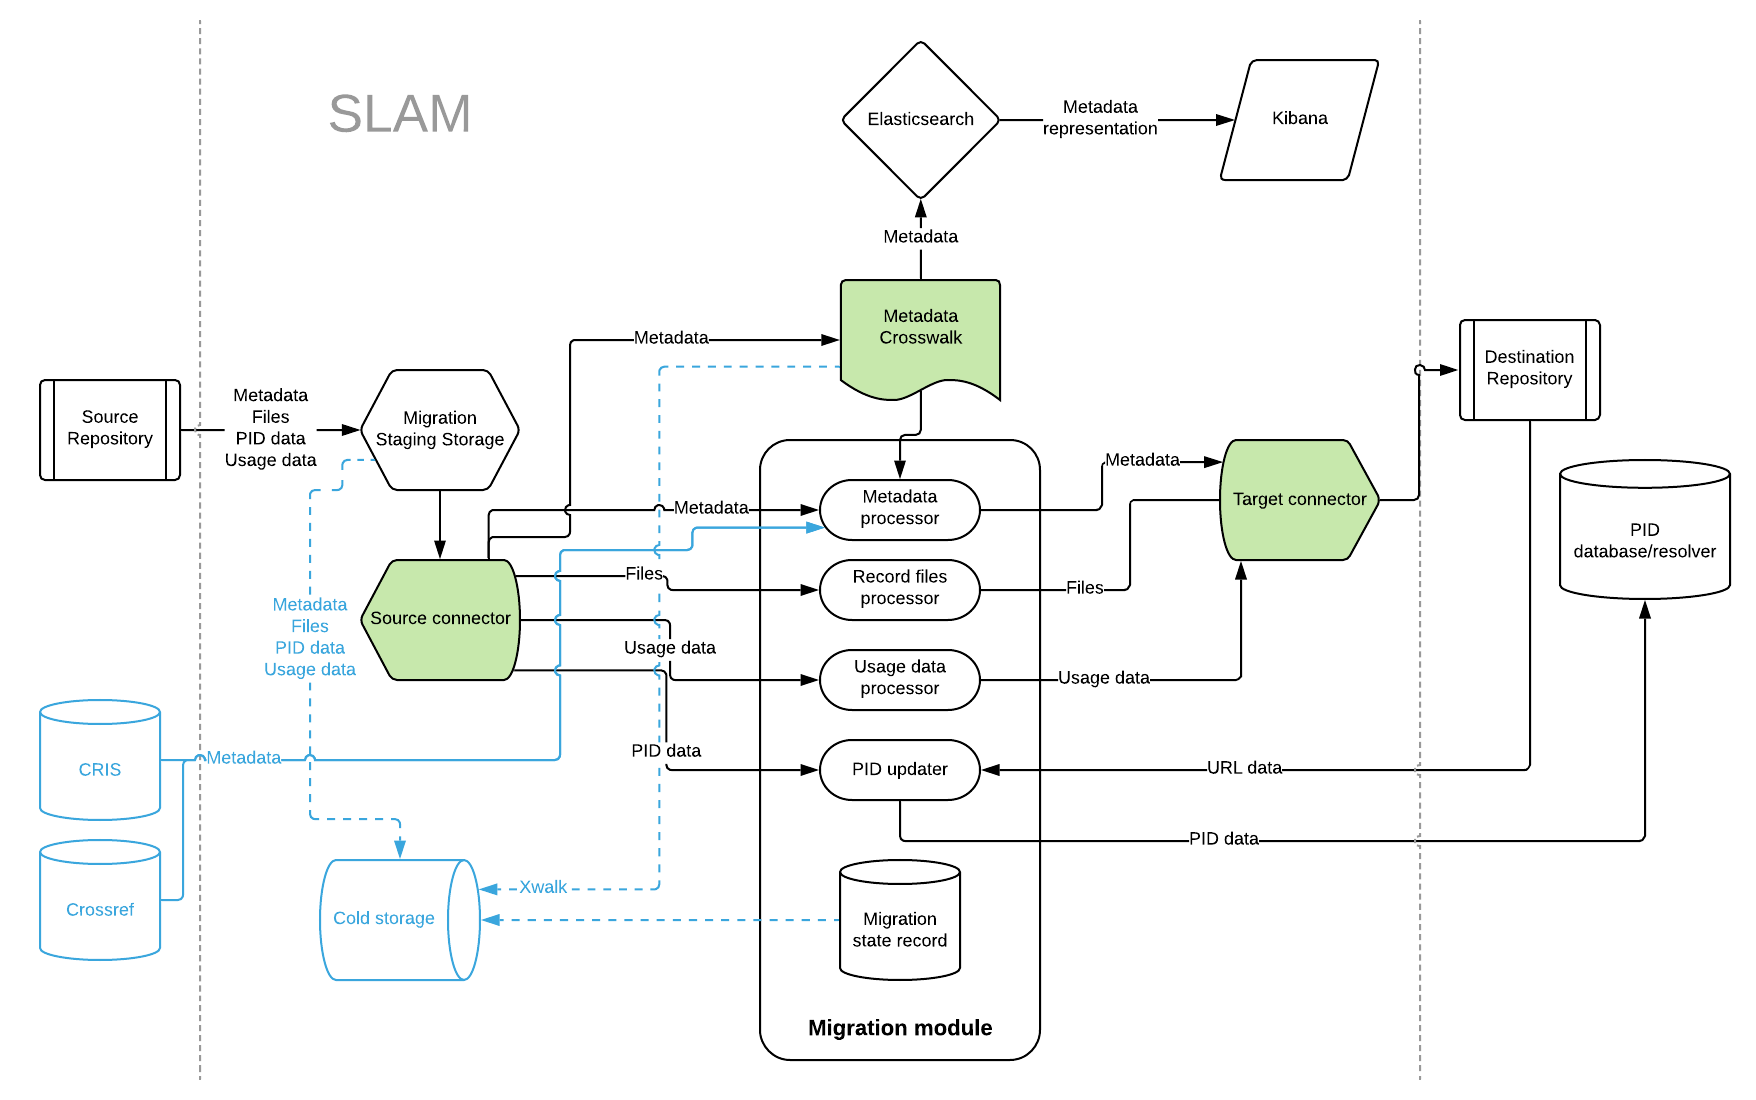
\includegraphics[scale=0.68]{figures/flow.png}}
  \caption{Main components and data flow in SLAM. The system splits the data to be migrated in four logical slices: bibliographic metadata, record files (e.g., \gls{pdf} journal articles), persistent identifiers of records, and usage data (views and downloads). A crosswalk is defined for the metadata and analysed using an Elasticsearch based setup in order to identify potential inconsistencies. The current state of the migration is recorded in a special file, in order to allow for multiple idempotent runs. Metadata can be enriched using external sources, such as a \gls{cris}, or open registries such as Crossref. All migration data is preserved for future reference. Areas in light blue are currently under development. The components highlighted in green need to be adapted for each migration.}
  \label{fig:workflow}
\end{sidewaysfigure}
\afterpage{\clearpage}

The first step concerns extracting all the required information from the source repository. This could be achieved in multiple ways, such as harvesting through an \gls{oai}-\gls{pmh} endpoint or other types of \glspl{api}, using the bulk export functionality implemented by most repository systems, or even by crawling the \gls{html} markup describing records, similar to how search engines do in order to discover web pages. Once this mechanism has been established, practical experience proved that it is beneficial to move this raw data \emph{closer} to the destination repository (to a \emph{staging} area as depicted in Fig. \ref{fig:workflow}). While this transfer might prove cumbersome, especially for large corpora, the operation is required only once. Moreover, having the data close to the destination repository allows faster prototyping and testing of the migration procedure, as network latency and throughput are improved\footnote{This assumes that SLAM is also deployed close to the target repository and the staging storage.}, while also ensuring that the source repository's functioning is not affected in any manner.

Metadata is the first considered aspect; from the migration's point of view, two dimensions are considered, the syntax and the semantics. As discussed in previous chapters, metadata comes in various formats, such as \gls{csv} or \gls{xml} files, and most of these can be easily parsed by openly available software solutions. Of more interest are the semantics of metadata, which stem from the employed \emph{schemas}, such as \gls{dcmt} or DataCite. A schema crosswalk which describes how the fields in the target repository schema should be populated using the source data needs to be set up when transferring records. While this should not be a concern if the two repositories use the same schema, for the performed migrations this was not the case; other reasons for setting up such a crosswalk include:
\begin{enumerate}
    \item Loosely defined schema in at least one of the repositories: certain repository systems do no specify a schema with clear field definitions, validations or applicability. By having the source repository administrators help with setting up a crosswalk, the migration team can avoid issues caused by incomplete understanding of the metadata.
    \item Support the review of the bibliographic records: migrations can prove to be an opportunity for reviewing and amending the records' metadata; for example, infrequently used fields can be completely removed and values which tend to confuse end-users can be moved to other fields.
    \item Ensure that a record on how the migration was performed, from the metadata point of view, is maintained. The crosswalk is considered an output of the migration and is preserved for future reference. 
\end{enumerate}

The crosswalk is tested using Elasticsearch, \emph{``an open source search and analytics engine for all types of data, including textual, numerical, geospatial, structured, and unstructured''}\cite{elastic}. The setup uses the crosswalk to create Elasticsearch \emph{documents} which include all fields as they would be transferred to the destination repository. A Kibana dashboard\footnote{\url{https://www.elastic.co/products/kibana}} is then used to both visually inspect the records and also to enable structured searches across the corpus. This can allow, for example, discovering fields which do not follow a consistent pattern for the values, as the example in Fig. \ref{fig:kibana}. As the crosswalk includes, apart from the field mapping, altering operations that can be performed on each field (e.g., using a standard format for all dates), this analysis can facilitate the review process described by the second point above. While performing actual migrations, a number of inconsistencies about which the source repository administrators were unaware of have been surfaced by SLAM and corrected in the target repository; this is common-place especially in large corpora spanning multiple decades, where the repository metadata workflows and schemas might have changed multiple times.

\begin{figure}[ht!]
  \centering
  \fbox{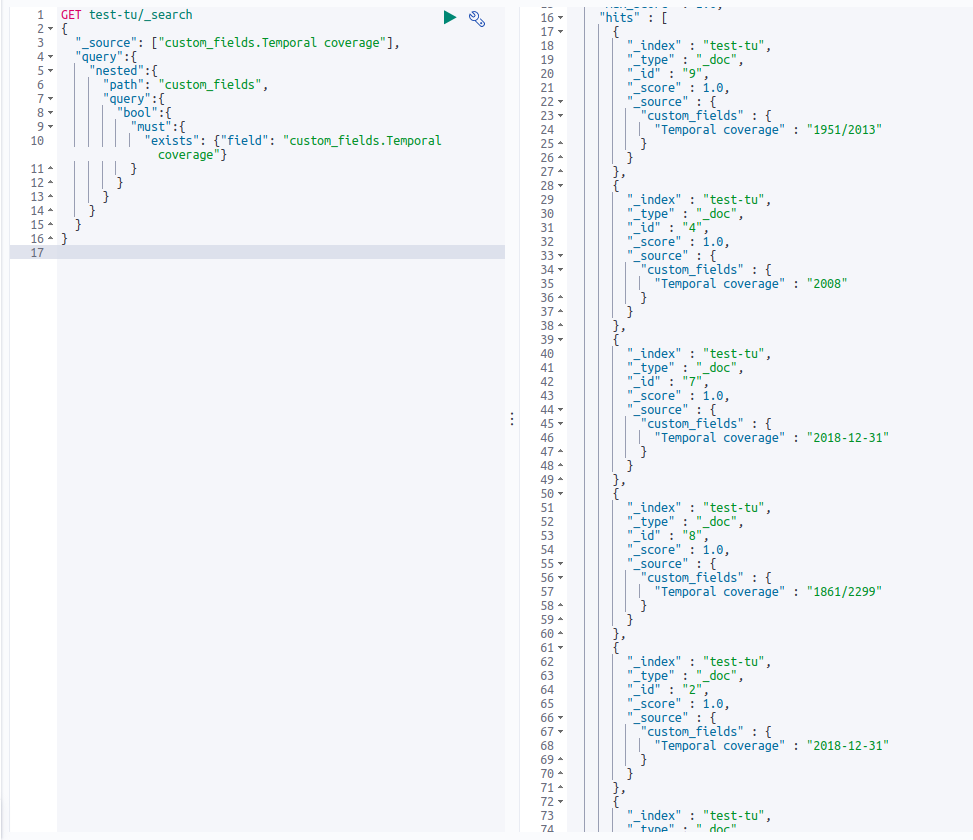
\includegraphics[scale=0.43]{figures/temporal.png}}
  \caption{A view examining the possible values of the temporal coverage field from the Dublin Core schema in a migrated institutional repository corpus. This shows variation in the format of the values (full date, year-only) which can cause issues if migrated to a schema which applies strict validation on date/time values and thus need to be handled by the migration harness. This view is generated using Kibana from the Elasticsearch stack, employed by SLAM for metadata analysis purposes.} 
  \label{fig:kibana}
\end{figure}

Two points should be noted about this component:
\begin{itemize}
    \item This is the only component of the architecture for which an actual implementation is mentioned, namely Elasticsearch. While other solutions could have been chosen, such as the ones included in the Bridge2Hyku toolkit\cite{bridge} (e.g., OpenRefine\footnote{\url{http://openrefine.org/}}), Elasticsearch proved to be the best fit for a highly automated system which requires analysis capabilities; it is a production-grade solution which can index high number of documents and support complex queries, while also providing user-friendly analytical views via Kibana.
    \item Arguments for loading the metadata in the analysis component \emph{without} having it processed through the crosswalk can be brought; such a workflow could provide further insights into various issues of the corpus which are possibly obscured by the crosswalk. The practical experiences of this project did not uncover any such issues, while this specific implementation provided a mean to test the crosswalk, a major migration component; nevertheless, the possibility of having all the raw metadata loaded into an analysis tool before performing any mutation on it needs to be considered for other migrations. It is worth noting that in such cases Elasticsearch might not be the best fit, as due to its architecture it requires a \emph{mapping} in order to load and index documents\cite{mapping}; other solutions, such as Athena\footnote{\url{https://aws.amazon.com/athena/}} could replace it for the analysis component of SLAM.
\end{itemize}

With the crosswalk set up, the migration module can be completed. From a logical point of view, it comprises of four components:
\begin{enumerate}
    \item Metadata processing: this component uses the crosswalk in order to transfer the metadata to the target repository.
    \item File upload: this simply uploads all files associated to a bibliographic record to their new location.
    \item Usage data transfer: most repositories nowadays implement counters for views and downloads of records, and this information, if available, is also transferred to the target repository.
    \item Persistent identifier update: if the records were using \glspl{pid}, such as \glspl{doi}, these are updated to \emph{resolve} to the new locations on the target repository. While the usage of \glspl{pid} is desirable, even across the migrations performed by using SLAM a number of cases where persistent identifiers were not employed were encountered; records were accessible only via \glspl{uri} and these cannot always be transferred between repositories, as each software usually uses its own schema. As this poses an issue for the continuity and preservation of records, implementing identifiers is highly advised before performing a repository migration.
\end{enumerate}

One of the architectural goals of SLAM is idempotence and this is implemented at migration's module level, which is designed as a state machine. A trivial example of such a state machine is included in Fig. \ref{fig:state}. The state machine status is serialised in a persistent database (the current implementation uses a \gls{json} format for state serialisation), each migration run deserialising it in order to determine which operations still need to be applied for each record. Maintaining such a registry provides a number of other benefits:
\begin{itemize}
    \item Facilitates testing and prototyping: this was the original reason behind the architecture, useful especially before the metadata analysis functionality was implemented. If one of the operations required for transferring a record fails, subsequent runs will not require to apply all steps, but only the ones that did not complete. As for each record a separate state section is maintained\footnote{Practical experiences proved that the best way of identifying records is by their unique identifier in the source repository, especially when no universal persistent identifiers are present.}, this becomes especially useful when migrating multiple entries; records which failed to migrate can be easily isolated and subsequently reprocessed.
    \item Allows creating reports on the migration; these are used, for example, to validate that all records were indeed transferred to the target repository.
    \item The migration module becomes portable; as long as the state machine serialisation is accessible, the module can run from different systems and at different points in time.
\end{itemize}

\begin{figure}[ht!]
  \centering
  \fbox{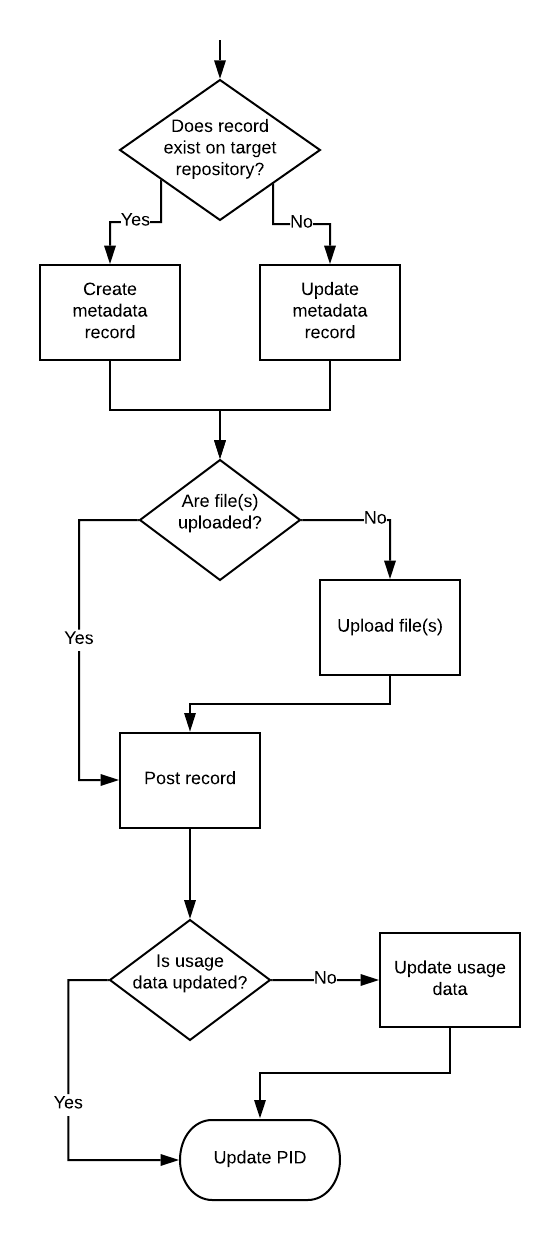
\includegraphics[scale=0.7]{figures/state.png}}
  \caption{A simplified process diagram for migrating a record. Each successful operation is recorded in a persistent database which is used in subsequent runs for deciding the workflow path. For example, files will not be uploaded each time the migration script is ran, thus avoiding duplication.} 
  \label{fig:state}
\end{figure}

The first architectural principle previously presented relates to the reusability of SLAM across migrations. The most common cause of divergence between migrations is related to the differences between repository solutions; SLAM isolates this concern by using two \emph{connectors}, one for the source and one for the target repository. These connectors translate the information to be migrated to and from SLAM's internal data model. Thus, the source connector needs to be able to traverse the staging storage and provide SLAM with all the required record information, while the target connector will upload the records to the new repository (using an \gls{http}-accessible \gls{api} for example). This means that for each migration only 3 parts of SLAM need to be adapted (green highlights in Fig. \ref{fig:workflow}): the source and target connectors, and the metadata crosswalk. All other components can remain unchanged, thus reducing the technical development time.

In the last step of SLAM's workflow the information that was used for the migration is sent to a long-term preservation storage, in order to ensure that it remains available for future reference. In the current implementation, the following information is preserved:
\begin{itemize}
    \item Original metadata and files, as extracted from the source repository;
    \item Metadata crosswalk;
    \item Migration script state machine serialization.
\end{itemize}
This information is sufficient for understanding the exact steps applied during the migration and, if required, for applying certain corrections to the migrated records at a future point in time.


\section{Evaluation of SLAM}
\label{sec:eval}

SLAM was used for performing five repository migrations during one year, as described in Table \ref{tbl:migrations}; the target repository in all five cases was Figshare. 
\begin{table}[thpb]
\centering
\begin{tabular}{|c||c|c|c|}
\hline
\specialcell{Source\\repository\\identifier} & \specialcell{Repository\\type} & Software & \specialcell{Number of\\records}\\ 
\hline\hline
IR1 & Institutional & DSpace & $37.000$ \\ \hline
IR2 & Institutional & DSpace & $25.605$ \\ \hline
D1 & Data & Custom & $334$ (105 GB) \\ \hline
IR3 & Institutional & Digital Commons & $2.275$ \\ \hline
IR4 & Institutional & DSpace & $15.474$ \\ \hline
\end{tabular}
\caption{Overview of repositories migrated to Figshare using SLAM.}
\label{tbl:migrations}
\end{table}

SLAM's viability was assessed based on the design principles outlined at the beginning of the chapter. Reusability, the main rationale behind SLAM, relates to being able to reuse as much of the system as possible across migrations. The architecture isolated the parts that required adaption from one migration to another (the connectors and the crosswalk); the time spent by a software engineer in order to set up these was monitored. The target here was to support the specialised staff on making domain-specific decisions, especially on the metadata crosswalk\footnote{An example here are the strict metadata requirements around the Research Excellence Framework (REF) 2021 exercise in the United Kingdom, which require thorough testing in connection with \gls{cris} and \gls{oa} monitoring solutions.}, by reducing the time spent developing the three mentioned components. Between IR1 and IR4 this was reduced from six \emph{man-weeks} to only two; it is important to note that SLAM evolved between the migrations, based on the lessons learned from each instance. 
    
Idempotence, allowing the re-processing of migrated records, is covered in SLAM by the state machine implemented in the migration module, which is persistent and can be referenced in subsequent runs. All the migrations in Table \ref{tbl:migrations} required supplementary runs after all records were migrated, most frequently in order to fix metadata issues discovered after the full corpus was transferred. For example, IR1 required three such runs:
\begin{enumerate}
    \item First run fixed a number of issues caused by omissions in the metadata schema crosswalk.
    \item The second run enriched the metadata using information taken from a \gls{cris}.
    \item The last run corrected the usage statistics (view and downloads) which were incorrectly imported initially, due to incomplete understanding of the source repository database.
\end{enumerate}
Due to SLAM's design, no issues were encountered while performing these runs, as no records were duplicated, removed or erroneously modified. A key aspect highlighted by the requirement to reprocess migrated records relates to the granularity of the state machine. As an example, in IR3 a second run required attaching supplementary files to a number of migrated records, and this posed a challenge due to the fact that the state machine only recorded if \emph{all} files have been uploaded, and not \emph{which} files were successfully added to the record. Thus, this state was amended in order to record the complete list of record files, allowing for more granular control over this processing step. 
    
The last concern, fault tolerance, was achieved by applying basic software engineering principles, such as \emph{fail-fast} (report migration issues as soon as they manifest), the implementation of proper exception handling (such as not to ignore any potential issues while also allowing SLAM to run after encountering issues on a particular record), and addition of enhanced logging in order to provide a complete detailed view of the processing steps. For each of the five migrations, SLAM ran unsupervised, reporting at the end of each run the records for which an issue was encountered; as an example, in the IR4 migration, SLAM initially failed to migrate 300 records; these were reported to the operator, and after minor fixes were applied to the metadata crosswalk the migration completed successfully. Fault-tolerance plays a central role in ensuring that during migrations no data is lost or corrupted, by surfacing any \emph{edge-case} that might have been missed during the development of the metadata crosswalk, repository connectors, or core migration module, while also isolating such issues to the records exhibiting them, with no impact on the full corpus. 

While proven viable in real-world scenarios, SLAM's design includes a number of areas which can benefit from further improvements. An analysis of the current implementation, based on the experiences of the five migrations, uncovered four such areas.

First, the migration-specific components (connectors and metadata crosswalk, in green in Fig. \ref{fig:workflow}) require further decoupling from the core migration module. For example, due to the fact that all migrations considered Figshare as a target repository, this connector is currently strongly interlinked with the core module, in order to save development time according to business requirements and migration timelines. Further decoupling will ensure that the core migration module's design is not influenced in any way by the repository's architecture and capabilities.

Further to this point, the metadata crosswalk is currently influenced by the logic and design of the migration module; for example, it uses the same procedural programming language, Python. Employing technologies such as \gls{xslt} or SPARQL (for \gls{rdf}) will help involve staff with in-depth domain knowledge further in the migration, as these technologies are more familiar and such a design does not require any knowledge of SLAM's internal processes.

Second, the five performed migrations highlighted the importance of reviewing, correcting and enhancing records during the migration. For example, when migrating a journal article's version of record in an \gls{oa} context, special care needs to be given to its metadata (title, authors, journal name, publication date), as mistakes can generate issues with scholarly search engines which aim to link the publisher version to the repository one. A possible source for comparing and correcting existing metadata is the information contained by a \glspl{cris}, which aggregates information from various databases (e.g., Scopus\footnote{\url{https://www.scopus.com/}}). If access to such systems is not available, it is possible to source metadata from open directories, such as Crossref.

The third area in need of improvement relates to testing the final outcome of the migration. Currently, repository administrators need to visually inspect the records in the target repository (either a representative sample or the full corpus), and this can be both cumbersome and error-prone. While in line with SLAM's philosophy of automating every step of the process, implementing a mechanism for validating the end migration result could also provide stronger assurances on the completeness and correctness of the migration. Again, using techniques specific to software engineering, such as unit testing, can prove helpful. In the absence of automated solutions, more systematic approaches can be considered; for example, in \cite{denney} the authors selected at random a representative sample of results from an \gls{etl} workload and manually compared them to their sources, in order to validate the correctness of the transformations.

Finally, SLAM's preservation module requires further development in order to ensure that it is fully automated; moreover, the possibility of adding a \emph{manifest} explaining the migration outputs needs to be considered, as knowledge on the organisation of the information, which is specific to each migration, might be lost in time.

It is important to note that architecture-wise, which was the main concern of this work, no major shortcomings in SLAM were identified, most issues above relating to implementation details. SLAM's modular design will facilitate any additions to the system, required in order to support new use cases and migrations.

To sum up, the main contributions brought by SLAM are:
\begin{enumerate}
    \item It includes an analysis module based on an industry standard search engine, Elasticsearch, which allows operators to analyse the metadata and schema crosswalk, facilitating the decisions required for properly migrating information between repositories.
    \item It implements a serialisable state machine in its migration module, which facilitates running the same migration multiple times without duplicating, removing or corrupting records, while allowing for corrections to be applied to the corpus.
    \item It follows a modular design, which enhances its reusability across multiple migrations by reducing the development time required for adapting the system to new source and target repositories.
\end{enumerate}

SLAM applies established software engineering principles in order to provide a trustworthy tool to digital library administrators that need to transfer content between such systems. Its design was both influenced and validated by real-world applications, having been used for five different migrations with various requirements and targeted repository solutions. Future work needs to consider enhancing SLAM's metadata analysis and enrichment capabilities while also collecting further data points on its performance and possible improvement directions while using it for other respository migrations.